\documentclass[tikz]{standalone}

\usepackage[latin1]{inputenc}
\usepackage{tikz}

% GNUPL
\begin{document}
\pagestyle{empty}
\newcommand\spiral{}% Just for safety so \def won't overwrite something
\def\spiral[#1](#2)(#3:#4:#5){% \spiral[draw options](placement)(end angle:revolutions:final radius)
\pgfmathsetmacro{\domain}{pi*#3/180+#4*2*pi}
\draw [#1,shift={(#2)}, domain=0:-\domain,variable=\t,samples=int(\domain/0.08)] plot ({\t r}: {#5*\t/\domain})
}
\def\spirall[#1](#2)(#3:#4:#5){% \spiral[draw options](placement)(end angle:revolutions:final radius)
\pgfmathsetmacro{\domain}{pi*#3/180+#4*2*pi}
\draw [#1,shift={(#2)}, domain=0:\domain,variable=\t,samples=int(\domain/0.08)] plot ({\t r}: {#5*\t/\domain})
}

\usetikzlibrary{decorations.pathreplacing,decorations.markings,arrows}
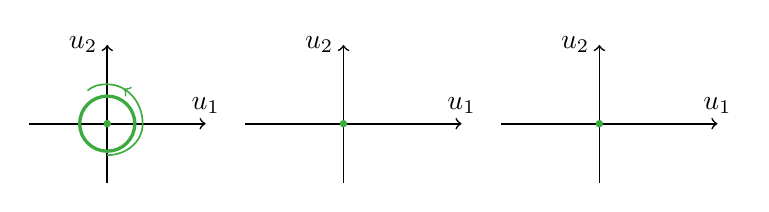
\begin{tikzpicture}[scale=0.5]
    %\mu<0
    
    \draw[semithick] [->] (0.5,2) -- (5,2) node[above] {$u_1$};
    \draw[semithick] [->] (2.5,0.5) -- (2.5,4) node[left] {$u_2$};
    \spiral[semithick, 
            postaction={decorate,
                decoration={markings,mark=at position 0.95 with {\arrow{<}}}
               },
     color={rgb,255:red,60; green,170; blue,60}](2.5,2)(75:2:0.5);
      %цвет влюбленной жабы
    \draw [fill, color={rgb,255:red,60; green,170; blue,60}] (2.5,2) circle [radius=0.08];
    \draw [very thick, color={rgb,255:red,60; green,170; blue,60}] (2.5,2) circle [radius=0.7];
    \draw [color={rgb,255:red,60; green,170; blue,60}, semithick] (2.5,1.2) to [out=0,in=-90] (3.4,2) to [out=90,in=0] (2.5,3) to [out=180,in=40] (2,2.84);
    \draw [color={rgb,255:red,60; green,170; blue,60}, semithick] [->] (3,2.836) --(2.92,2.89);
  %\mu=0
    \draw[semithick] [->] (6,2) -- (11.5,2) node[above] {$u_1$};
    \draw[semithick] [->] (8.5,0.5) -- (8.5,4) node[left] {$u_2$};
    \spirall[semithick, 
            postaction={decorate,
                decoration={markings,mark=at position 0.95 with {\arrow{>}}}
               },
     color={rgb,255:red,60; green,170; blue,60}](8.5,2)(10:5:1.5); 
     \draw [fill, color={rgb,255:red,60; green,170; blue,60}] (8.5,2) circle [radius=0.08];
    %\mu>0
    
    \draw[semithick] [->] (12.5,2) -- (18,2) node[above] {$u_1$};
    \draw[semithick] [->] (15,0.5) -- (15,4) node[left] {$u_2$};
    \spirall[semithick, 
            postaction={decorate,
                decoration={markings,mark=at position 0.95 with {\arrow{>}}}
               },
     color={rgb,255:red,60; green,170; blue,60}](15,2)(10:2.5:1.5); 
     \draw [fill, color={rgb,255:red,60; green,170; blue,60}] (15,2) circle [radius=0.08];
\end{tikzpicture}
\end{document}